\documentclass[a4paper,12pt,twoside]{memoir}

\setsecnumdepth{subsection}

% Castellano
\usepackage[spanish,es-tabla]{babel}
\selectlanguage{spanish}
\usepackage[utf8]{inputenc}
\usepackage[T1]{fontenc}
\usepackage{lmodern} % Scalable font
\usepackage{microtype}
\usepackage{placeins}
\usepackage{dirtree}

\RequirePackage{booktabs}
\RequirePackage[table]{xcolor}
\RequirePackage{xtab}
\RequirePackage{multirow}

% Links
\usepackage[colorlinks]{hyperref}
\hypersetup{
	allcolors = {red}
}

% Ecuaciones
\usepackage{amsmath}

% Rutas de fichero / paquete
\newcommand{\ruta}[1]{{\sffamily #1}}

% Párrafos
\nonzeroparskip

% Huérfanas y viudas
\widowpenalty100000
\clubpenalty100000

% Evitar solapes en el header
\nouppercaseheads

% Imagenes
\usepackage{graphicx}
\newcommand{\imagen}[2]{
	\begin{figure}[!h]
		\centering
		\includegraphics[width=0.9\textwidth]{#1}
		\caption{#2}\label{fig:#1}
	\end{figure}
	\FloatBarrier
}

\newcommand{\imagenflotante}[2]{
	\begin{figure}%[!h]
		\centering
		\includegraphics[width=0.9\textwidth]{#1}
		\caption{#2}\label{fig:#1}
	\end{figure}
}



% El comando \figura nos permite insertar figuras comodamente, y utilizando
% siempre el mismo formato. Los parametros son:
% 1 -> Porcentaje del ancho de página que ocupará la figura (de 0 a 1)
% 2 --> Fichero de la imagen
% 3 --> Texto a pie de imagen
% 4 --> Etiqueta (label) para referencias
% 5 --> Opciones que queramos pasarle al \includegraphics
% 6 --> Opciones de posicionamiento a pasarle a \begin{figure}
\newcommand{\figuraConPosicion}[6]{%
  \setlength{\anchoFloat}{#1\textwidth}%
  \addtolength{\anchoFloat}{-4\fboxsep}%
  \setlength{\anchoFigura}{\anchoFloat}%
  \begin{figure}[#6]
    \begin{center}%
      \Ovalbox{%
        \begin{minipage}{\anchoFloat}%
          \begin{center}%
            \includegraphics[width=\anchoFigura,#5]{#2}%
            \caption{#3}%
            \label{#4}%
          \end{center}%
        \end{minipage}
      }%
    \end{center}%
  \end{figure}%
}

%
% Comando para incluir imágenes en formato apaisado (sin marco).
\newcommand{\figuraApaisadaSinMarco}[5]{%
  \begin{figure}%
    \begin{center}%
    \includegraphics[angle=90,height=#1\textheight,#5]{#2}%
    \caption{#3}%
    \label{#4}%
    \end{center}%
  \end{figure}%
}
% Para las tablas
\newcommand{\otoprule}{\midrule [\heavyrulewidth]}
%
% Nuevo comando para tablas pequeñas (menos de una página).
\newcommand{\tablaSmall}[5]{%
 \begin{table}
  \begin{center}
   \rowcolors {2}{gray!35}{}
   \begin{tabular}{#2}
    \toprule
    #4
    \otoprule
    #5
    \bottomrule
   \end{tabular}
   \caption{#1}
   \label{tabla:#3}
  \end{center}
 \end{table}
}

%
% Nuevo comando para tablas pequeñas (menos de una página).
\newcommand{\tablaSmallSinColores}[5]{%
 \begin{table}[H]
  \begin{center}
   \begin{tabular}{#2}
    \toprule
    #4
    \otoprule
    #5
    \bottomrule
   \end{tabular}
   \caption{#1}
   \label{tabla:#3}
  \end{center}
 \end{table}
}

\newcommand{\tablaApaisadaSmall}[5]{%
\begin{landscape}
  \begin{table}
   \begin{center}
    \rowcolors {2}{gray!35}{}
    \begin{tabular}{#2}
     \toprule
     #4
     \otoprule
     #5
     \bottomrule
    \end{tabular}
    \caption{#1}
    \label{tabla:#3}
   \end{center}
  \end{table}
\end{landscape}
}

%
% Nuevo comando para tablas grandes con cabecera y filas alternas coloreadas en gris.
\newcommand{\tabla}[6]{%
  \begin{center}
    \tablefirsthead{
      \toprule
      #5
      \otoprule
    }
    \tablehead{
      \multicolumn{#3}{l}{\small\sl continúa desde la página anterior}\\
      \toprule
      #5
      \otoprule
    }
    \tabletail{
      \hline
      \multicolumn{#3}{r}{\small\sl continúa en la página siguiente}\\
    }
    \tablelasttail{
      \hline
    }
    \bottomcaption{#1}
    \rowcolors {2}{gray!35}{}
    \begin{xtabular}{#2}
      #6
      \bottomrule
    \end{xtabular}
    \label{tabla:#4}
  \end{center}
}

%
% Nuevo comando para tablas grandes con cabecera.
\newcommand{\tablaSinColores}[6]{%
  \begin{center}
    \tablefirsthead{
      \toprule
      #5
      \otoprule
    }
    \tablehead{
      \multicolumn{#3}{l}{\small\sl continúa desde la página anterior}\\
      \toprule
      #5
      \otoprule
    }
    \tabletail{
      \hline
      \multicolumn{#3}{r}{\small\sl continúa en la página siguiente}\\
    }
    \tablelasttail{
      \hline
    }
    \bottomcaption{#1}
    \begin{xtabular}{#2}
      #6
      \bottomrule
    \end{xtabular}
    \label{tabla:#4}
  \end{center}
}

%
% Nuevo comando para tablas grandes sin cabecera.
\newcommand{\tablaSinCabecera}[5]{%
  \begin{center}
    \tablefirsthead{
      \toprule
    }
    \tablehead{
      \multicolumn{#3}{l}{\small\sl continúa desde la página anterior}\\
      \hline
    }
    \tabletail{
      \hline
      \multicolumn{#3}{r}{\small\sl continúa en la página siguiente}\\
    }
    \tablelasttail{
      \hline
    }
    \bottomcaption{#1}
  \begin{xtabular}{#2}
    #5
   \bottomrule
  \end{xtabular}
  \label{tabla:#4}
  \end{center}
}



\definecolor{cgoLight}{HTML}{EEEEEE}
\definecolor{cgoExtralight}{HTML}{FFFFFF}

%
% Nuevo comando para tablas grandes sin cabecera.
\newcommand{\tablaSinCabeceraConBandas}[5]{%
  \begin{center}
    \tablefirsthead{
      \toprule
    }
    \tablehead{
      \multicolumn{#3}{l}{\small\sl continúa desde la página anterior}\\
      \hline
    }
    \tabletail{
      \hline
      \multicolumn{#3}{r}{\small\sl continúa en la página siguiente}\\
    }
    \tablelasttail{
      \hline
    }
    \bottomcaption{#1}
    \rowcolors[]{1}{cgoExtralight}{cgoLight}

  \begin{xtabular}{#2}
    #5
   \bottomrule
  \end{xtabular}
  \label{tabla:#4}
  \end{center}
}


\graphicspath{ {./img/} }

% Capítulos
\chapterstyle{bianchi}
\newcommand{\capitulo}[2]{
	\setcounter{chapter}{#1}
	\setcounter{section}{0}
	\chapter*{#2}
	\addcontentsline{toc}{chapter}{#1. #2}
	\markboth{#2}{#2}
}

% Apéndices
\renewcommand{\appendixname}{Apéndice}
\renewcommand*\cftappendixname{\appendixname}

\newcommand{\apendice}[1]{
	%\renewcommand{\thechapter}{A}
	\chapter{#1}
}

\renewcommand*\cftappendixname{\appendixname\ }

% Formato de portada
\makeatletter
\usepackage{xcolor}
\newcommand{\tutor}[1]{\def\@tutor{#1}}
\newcommand{\cotutor}[1]{\def\@cotutor{#1}}
\newcommand{\course}[1]{\def\@course{#1}}
\definecolor{cpardoBox}{HTML}{E6E6FF}
\def\maketitle{
	\null
	\thispagestyle{empty}
	% Cabecera ----------------
	\begin{center}%
		{\noindent\LARGE Universidades de Burgos, León y Valladolid}\vspace{.5cm}%
		
		{\noindent\large Máster universitario}\vspace{.5cm}%
		
		{\noindent\LARGE \textbf{Inteligencia de Negocio y Big~Data en Entornos Seguros}}\vspace{.5cm}%
	\end{center}%
	
	\begin{center}%
		
\includegraphics[height=3cm]{img/escudoUBU} \hspace{1cm}
		
\includegraphics[height=3cm]{img/escudoUVA} \hspace{1cm}
		
\includegraphics[height=3cm]{img/escudoULE} \vspace{1cm}%
	\end{center}%
	
	\vfill
	% Título proyecto y escudo informática ----------------
	\colorbox{cpardoBox}{%
		\begin{minipage}{.9\textwidth}
			\vspace{.4cm}\large
			\begin{center}
				\textbf{TFM del Máster Inteligencia de Negocio y Big Data en Entornos Seguros}\vspace{.6cm}\\
				\textbf{\Large\@title{}}
			\end{center}
			\vspace{.2cm}
		\end{minipage}
		
	}%
	\vfill
	% Datos de alumno, curso y tutores ------------------
	\begin{center}%
		{%
			\noindent\Large
			Presentado por \@author{}\\
			en la Universidad de Burgos --- \@date{}\\[1em]
			Tutores: Dr. \@tutor{} y\\\hspace{3.7em}Dr. \@cotutor{}
		}%
	\end{center}%
	\null
	\cleardoublepage
}
\makeatother

\newcommand{\nombre}{Iván Iglesias Cuesta} %%% cambio de comando
\newcommand{\titulo}{Uso de técnicas de aprendizaje no supervisado para la ayuda en videojuegos tipo MOBA}
\newcommand{\nombretutor}{José Francisco Díez Pastor}
\newcommand{\nombrecotutor}{César Ignacio García Osorio}

% Datos de portada
\title{\titulo}
\author{\nombre}
\tutor{\nombretutor}
\cotutor{\nombrecotutor}
\date{\today}

\begin{document}

\maketitle


\newpage\null\thispagestyle{empty}\newpage


%%%%%%%%%%%%%%%%%%%%%%%%%%%%%%%%%%%%%%%%%%%%%%%%%%%%%%%%%%%%%%%%%%%%%%%%%%%%%%%%%%%%%%%%
\thispagestyle{empty}


\noindent
\begin{center}%
	{\noindent\Huge Universidades de Burgos, León y Valladolid}\vspace{.5cm}%

\begin{center}%
	
\includegraphics[height=3cm]{img/escudoUBU} \hspace{1cm}
	
\includegraphics[height=3cm]{img/escudoUVA} \hspace{1cm}
	
\includegraphics[height=3cm]{img/escudoULE} \vspace{1cm}%
\end{center}%

	{\noindent\Large \textbf{Máster universitario en Inteligencia de Negocio y Big~Data en Entornos Seguros}}\vspace{.5cm}%
\end{center}%



\noindent D. \nombretutor, profesor del departamento de Ingeniería Informática, área de Lenguajes y Sistemas Informáticos.

\noindent D. \nombrecotutor, profesor del departamento de Ingeniería Informática, área de Lenguajes y Sistemas Informáticos.

\noindent Exponen:

\noindent Que el alumno D. \nombre, con DNI 45573756S, ha realizado el Trabajo final de Máster en Inteligencia de Negocio y Big Data en Entornos Seguros
          titulado \titulo.

\noindent Y que dicho trabajo ha sido realizado por el alumno bajo la dirección del que suscribe, en virtud de lo cual se autoriza su presentación y defensa.

\begin{center} %\large
En Burgos, {\large \today}
\end{center}

\vfill\vfill\vfill

% Author and supervisor
\begin{minipage}{0.45\textwidth}
\begin{flushleft} %\large
Vº. Bº. del Tutor:\\[2cm]
D. \nombretutor
\end{flushleft}
\end{minipage}
\hfill
\begin{minipage}{0.45\textwidth}
\begin{flushleft} %\large
Vº. Bº. del Tutor:\\[2cm]
D. \nombrecotutor
\end{flushleft}
\end{minipage}
\hfill

\vfill

% para casos con solo un tutor comentar lo anterior
% y descomentar lo siguiente
%Vº. Bº. del Tutor:\\[2cm]
%D. nombre tutor


\newpage\null\thispagestyle{empty}\newpage




\frontmatter

% Abstract en castellano
\renewcommand*\abstractname{Resumen}
\begin{abstract}
En este primer apartado se hace una \textbf{breve} presentación del tema que se aborda en el proyecto.
\end{abstract}

\renewcommand*\abstractname{Descriptores}
\begin{abstract}
MOBA, League of Legends, Riot Games, aprendizaje no supervisado, conjuntos frecuentes, ETL, Django, MongoDB.
\end{abstract}

\clearpage

% Abstract en inglés
\renewcommand*\abstractname{Abstract}
\begin{abstract}
A \textbf{brief} presentation of the topic addressed in the project.
\end{abstract}

\renewcommand*\abstractname{Keywords}
\begin{abstract}
MOBA, League of Legends, Riot Games, unsupervised items, frequent itemsets, ETL, Django, MongoDB.
\end{abstract}

\clearpage

% Indices
\tableofcontents

\clearpage

\listoffigures

\clearpage

\listoftables
\clearpage

\mainmatter

\addcontentsline{toc}{part}{Memoria}
\part*{Memoria}

\capitulo{1}{Introducción}

Las competiciones de deportes electrónicos, o \textit{esports}, al igual que los deportes tradicionales, mueven grandes cantidades de dinero a la vez que atraen a un número muy elevado de espectadores a sus retransmisiones.

Por lo general los juegos de los que se realizan competiciones son gratuitos, por lo que cualquier persona puede adentrarse en ese mundillo para pasar un rato entretenido, o ponerse la meta de llegar a ser profesional.

Sin embargo, esto es un objetivo complicado por la gran cantidad de horas necesarias para conseguir las capacidades necesarias para ser profesional. Además, el rango de edad en el que más necesario dedicar más horas de practica coincide con etapas de escolarización todavía obligatorias, pudiendo crear conflicto de intereses.

En ambos ámbitos, profesional y casual, se genera constantemente una gran cantidad de datos, tomando la forma de un registro de partidas jugadas. Para este trabajo me he propuesto analizar ese histórico de partidas en uno de los \textit{esports} más predominantes del momento, League of Legends, un videojuego dentro del tipo MOBA (\textit{Multiplayer Online Battle Arena}).

Mediante el uso de aprendizaje no supervisado, se puede extraer conocimiento del juego y ponerlo a disposición de las personas que empiezan a jugar y hacer más fácil esta entrada. Además de servir de ayuda en el ámbito profesional, para facilitar la preparación de un equipo ante una partida de competición.

\hfill
Ideas 
\begin{itemize}
    \item Importancia del mercado de los deportes electrónicos.
    \item Cifras de beneficios
    \item Cifras de espectadores
    \item https://newzoo.com/insights/trend-reports/newzoos-global-esports-live-streaming-market-report-2021-free-version/
    \item https://dotesports.com/league-of-legends/news/league-of-legends-reportedly-generated-1-75-billion-in-revenue-in-2020
    \item https://techacake.com/league-of-legends-player-count/
\end{itemize}
\capitulo{2}{Objetivos del proyecto}

Este apartado explica de forma precisa y concisa cuales son los objetivos que se persiguen con la realización del proyecto. Se puede distinguir entre los objetivos marcados por los requisitos del software a construir y los objetivos de carácter técnico que plantea a la hora de llevar a la práctica el proyecto.

\section{Objetivos principales}
\begin{itemize}
    \item Desarrollar un proceso ETL que sea capaz de recopilar los datos necesarios.
    \item Aplicar técnicas de aprendizaje no supervisado sobre los datos recopilados.
    \item Ser capaz de obtener conocimiento útil a partir de los datos obtenidos.
    \item Desarrollar una aplicación en la que se pueda consultar el conocimiento extraído.
    \item Que el producto final sea capaz de ayudar a los nuevos jugadores.
\end{itemize}


\section{Objetivos personales}
\begin{itemize}
    \item Aplicar lo aprendido durante el máster en un campo novedoso.
    \item Dar a conocer el mundo de los deportes electrónicos en un ambiente donde sean menos conocidos.
    \item Desarrollar un proyecto de ideación propia.
\end{itemize}
\capitulo{3}{Conceptos teóricos}

\section{ETL}
El término ETL (Extract, Transform, Load) se refiere al proceso de obtención de datos desde una o varias fuentes, su transformación y carga final en un lugar centralizado para su posterior uso.

\section{Aprendizaje no supervisado}
Dentro de la disciplina de aprendizaje automático, los algoritmos de aprendizaje no supervisado usan datos que no están clasificados o etiquetados previamente, con el objetivo de obtener las relaciones que existan entre los mismos. El tipo de algoritmos más conocidos de este grupo son los de \textit{clustering}, los cuáles se encargan de encontrar y clasificar las instancias de los datos de entrada en sus grupos correspodientes.

En este trabajo el tipo de algoritmos usados son los de conjuntos de elementos frecuentes. Estos son capaces de encontrar elementos que aparecen de forma conjunta frecuentemente en un gran listado de transacciones.

\section{Conceptos sobre \textit{League of Legends}}

\subsection{El juego}
\textit{League of Legends} es un videojuego de estrategia multijugador del tipo \textit{MOBA (Multiplayer Online Battle Arena)}, desarrollado por Riot Games y lanzado en 2011, en el que dos equipos de cinco jugadores se enfrentan para destruir la base del equipo enemigo \cite{misc:como-jugar}. Cada jugador controla dentro del juego a un personaje llamado campeón, que pueden seleccionar antes de empezar a jugar, y es único entre los diez jugadores.

Para asegurar la unicidad se lleva a cabo un proceso de selección de campeones (\ref{fig:early-pick}) entre los diez jugadores, ya divididos en dos equipos. Se empieza con una fase de prohibición, en la que cada jugador bloquea un campeón para evitar que se pueda jugar en la partida actual. Seguido se lleva a cabo la fase de selección, en la cual los jugadores van seleccionando su campeón en orden y alternando el equipo. Empieza el primer jugador del primer equipo, seguido van el primer y segundo jugador del segundo equipo, luego segundo y tercero del primer equipo, tercero y cuarto del segundo equipo, cuarto y quinto del primer equipo, y por último, quinto del segundo equipo.

\begin{figure}[h]
	\centering
	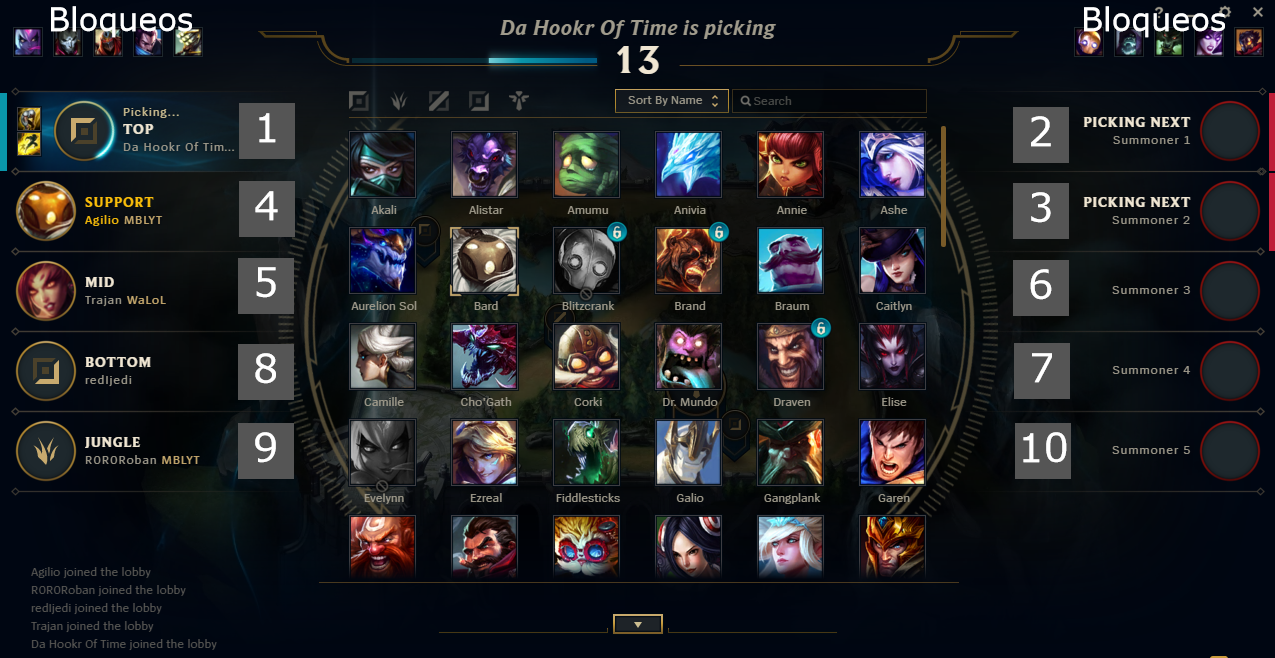
\includegraphics[width=1\linewidth]{img/early-pick}
	\caption{Proceso de selección de campeón}
	\label{fig:early-pick}
\end{figure}


Los jugadores se enfrentan en un mapa \ref{fig:mapa-lol} en forma de cuadrado, con las bases de cada equipo localizadas en zonas opuestas del mapa, una en la esquina inferior izquierda, y la otra en la superior derecha. Conectando cada base se encuentran tres líneas o calles, superior o \textit{top}, central o \textit{mid} e inferior o \textit{bot}. El espacio entre las calles se denomina jungla. Conectando las dos esquinas que no pertenecen a las bases se encuentra el río, que se encarga de separar el terreno del mapa dominado por cada equipo. De forma general los jugadores se reparten de la siguiente manera, uno en \textit{top}, uno en \textit{mid}, dos en \textit{bot} y el restante en la jungla.

\begin{figure}
	\centering
	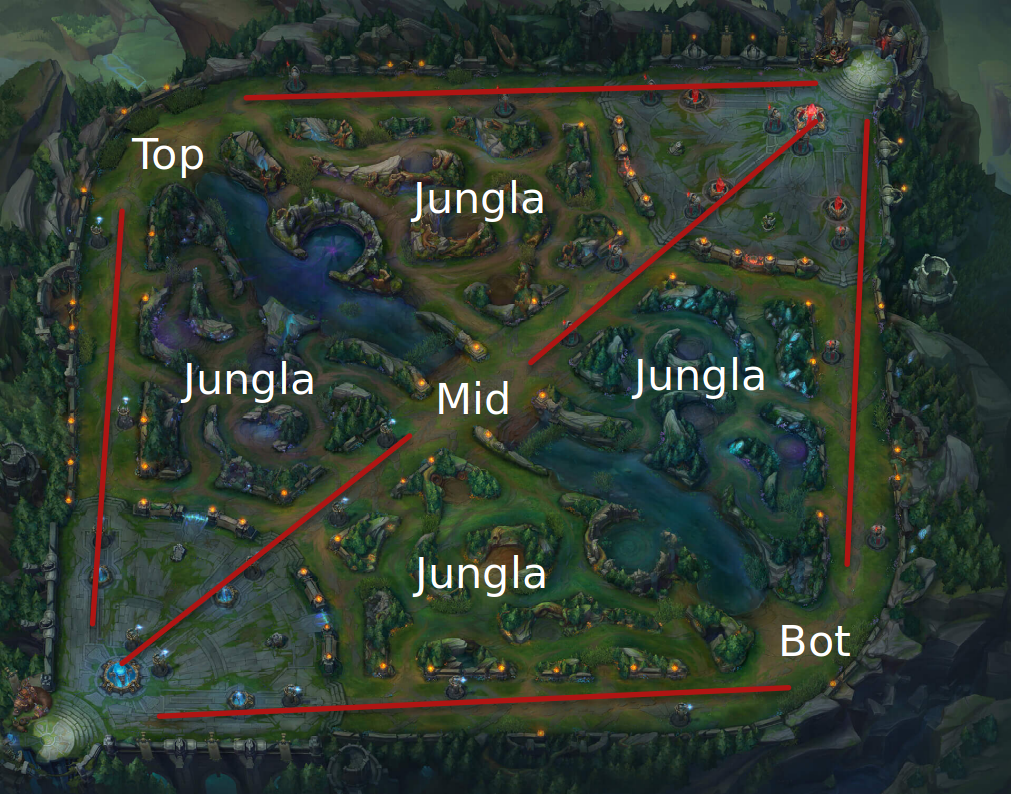
\includegraphics[width=1\linewidth]{img/mapa-lol}
	\caption{Mapa de \textit{League of Legends}.}
	\label{fig:mapa-lol}
\end{figure}

Para ganar la partida hay que destruir el nexo del equipo enemigo, es la estructura que está más alejada de la base propia. Las torres son otro tipo de estructuras situadas por el mapa, que disparan a los campeones del equipo contrario. Existen tres torres por cada línea y equipo, además de dos adicionales que protegen cada nexo. Las torres se tienen que derribar en el orden que se van encontrando en cada línea, y para destruir el nexo, como mínimo, hay que haber derribado todas las torres de una calle. Aunque un podría moverse por la jungla para llegar a cualquier torre, estas no reciben daño si la anterior sigue en pie.

La forma en la que un equipo consigue ventaja sobre el rival es mediante el oro, este se consigue de varias formas. La principal forma es asesinando a los campeones enemigos. Otras formas de conseguir oro es destruyendo las estructuras enemigas. La última forma de conseguir oro es matando monstruos y súbditos, los primeros se encuentran en la jungla, los segundos recorren las calles en oleadas. Tanto los campeones como los monstruos y súbditos vuelven a aparecen pasado un tiempo concreto, las estructuras una vez destruidas se mantienen así.

El oro permite comprar objetos, que mejoran las habilidades del campeón, haciendo que sea más sencillo derrotar a los campeones enemigos, lo que proporciona más oro para más objetos, causando un efecto bola de nieve y la eventual victoria del equipo.

Para ver estos conceptos de una forma más visual, Riot Games preparó un vídeo informativo de cara a los mundiales de 2020 para que la gente que no tuviera mucho conocimiento del juego y su funcionamiento pudiera ver y disfrutar la competición. El vídeo se titula \href{https://www.youtube.com/watch?v=ERkt_1TYlkU}{¿Así que queréis ver el Mundial? | Mundial 2020 - League of Legends}\footnote{\url{https://youtu.be/ERkt_1TYlkU}} y se encuentra disponible en YouTube.


\subsection{Campeones}
Los campeones son los diferentes personajes disponibles que un jugador puede seleccionar antes de la partida. Actualmente hay 156 disponibles, añadiéndose a la lista uno nuevo en franjas de tiempo que van desde uno a seis meses. Cada uno tiene un rol asignado que determina su forma de jugar, su función e incluso posición dentro del mapa. Los distintos roles son:
\begin{itemize}
	\tightlist
	\item Tirador
	\item Apoyo
	\item Asesino
	\item Luchador
	\item Tanque
	\item Mago
\end{itemize}

Para que un campeón acabe en una categoría u otra hay que prestar atención a varios factores, entre los que se encuentran su tipo de ataque básico, el efecto de sus habilidades y la forma en la que sus estadísticas modifican las habilidades. En las secciones \ref{habilidades} y \ref{estadisticas} se explican en detalles estos conceptos.

\subsection{Habilidades}
\label{habilidades}
Cada campeón tiene un conjunto único de habilidades, una pasiva y cuatro activas, se diferencian en que la pasiva está siempre causando un efecto y las activas causan su efecto cuando decide el jugador. Se pueden definir como las operaciones que un jugador puede realizar para interactuar con el mapa, con otros jugadores, monstruos y súbditos.

Cada habilidad puede tener un efecto o combinar varios, los cuales se aplican sobre uno mismo, un aliado o enemigo. Los efectos más comunes son las curaciones, realizar daños o control de adversario, donde se engloban ralentizaciones o inmovilizaciones. Estos efectos tienen unos valores numéricos que constan de dos partes, un valor base y uno variable que depende de las estadísticas del campeón.

Explicado con un ejemplo, una habilidad de un campeón hace daño a un enemigo con un valor base de 150 puntos de vida y un valor variable que corresponde al 30\% daño de ataque del campeón. Si en un momento determinado el campeón tiene 300 de daño de ataque, el daño total de la habilidad se calcula como $150 + (0,3 * 300) = 240$.

En el caso de realizar daño a un rival, existen tres formas en las que puede realizar: daño físico, mágico y verdadero. Esto está determinado por la habilidad y rol del campeón.

\subsection{Estadísticas}
\label{estadisticas}
Las estadísticas son diferentes valores numéricos que determinan las capacidades de cada campeón en un área en concreto del juego. Estos valores se ven modificados por la compra de objetos (\ref{objetos}). A continuación se describen las estadísticas y que representan.
\begin{description}
	\item[Daño de ataque] Daño realizado con ataques básicos.
	\item[Probabilidad de crítico] Probabilidad de que un ataque básico haga el doble de daño.
	\item[Velocidad de ataque] Cantidad de ataques básicos que se pueden realizar por segundo.
	\item[Poder de habilidad] Modifica el daño que realizan las habilidades.
	\item[Velocidad de movimiento] Velocidad a la que un campeón se desplaza por el mapa.
	\item[Armadura] Cantidad en la que se ve reducida el daño físico que se recibe.
	\item[Resistencia mágica] Cantidad en la que se ve reducida el daño mágico que se recibe.
	\item[Penetración de armadura] Cantidad de la armadura del rival ignorada a la hora de realizar daño físico.
	\item[Penetración mágica] Cantidad de la resistencia mágica del rival ignorada a la hora de realizar daño mágico.
	\item[Vida] Daño que tiene que recibir un personaje para morir.
	\item[Maná] Coste de usar habilidades.
	\item[Robo de vida] Porcentaje de vida recuperado al dañar a un rival.
\end{description}

\subsection{Objetos}
\label{objetos}
Dentro de la base de cada equipo en el mapa está localizada la tienda. Aquí los jugadores pueden comprar objetos con el oro que han ido ganando con el progreso de la partida. Su función es modificar las estadísticas del campeón, para que las habilidades del mismo sean más eficaces contra los rivales. Los objetos que se compran se quedan guardados en el inventario del campeón, el cual está limitado a seis objetos.

En el juego actual existen 222 objetos disponibles clasificados en cinco categorías:
\begin{description}
	\item[Iniciales] Objetos más relevantes al inicio de la partida, generalmente mejoran una estadística pero no pueden combinarse para formar un objeto de categoría superior.
	\item[Básicos] Objetos que mejoran una estadística.
	\item[Épicos] Objetos formados por la combinación de varios objetos básicos que mejoran varias estadísticas.
	\item[Legendarios] Objetos formados por la combinación de objetos épicos y/o básicos que mejoran varias estadísticas y proporcionan algún efecto adicional.
	\item[Míticos] Igual que los anteriores, pero limitado a uno en el inventario.
\end{description}

\subsection{Ligas}
Al igual que otros deportes, \textit{League of Legends} posee un sistema de ligas que clasifica a los jugadores que lo deseen dentro de su sistema de ligas, en base a la habilidad que demuestren en sus partidas.

En la tabla \ref{tab:ligas} se muestran las diferentes ligas disponibles ordenadas de menor a mayor habilidad. También se incluye el porcentaje de jugadores localizados en cada liga\cite{misc:player-distribution} y otros atributos explicados a continuación. El porcentaje no es fijo, los mostrados se refieren al estado de las ligas en agosto de 2021. Esto se debe al movimiento de jugadores entre ligas en base a las partidas que juegan y a los nuevos jugadores que empiecen a jugar.

Desde Hierro a Diamante, cada una cuenta con cuatro divisiones (subcategorías dentro de cada liga), que van desde IV a I. Las tres restantes tienen una única división. Además, tanto Gran Maestro como Aspirante tienen plazas limitadas, 700 y 300 respectivamente.

La localización de cada jugador se basa en un sistema de puntos, ganándolos al ganar partidas y perdiéndolos al perder. En las ligas con divisiones, cuando el jugador alcanza 100 puntos pasa a la siguiente división, o en el caso de estar en la divisón superior, subiría de liga. Por encima de Diamante no hay límite de puntos, y estando los jugadores ordenados por estos, la clasificación se realiza según el límite de plazas mencionado anteriormente.

\begin{table}[h]
	\begin{tabular}{c|c|c|c|c}
		\textbf{Nombre} & \textbf{Porcentaje} & \textbf{Divisiones} & \textbf{Límite usado} & \textbf{Cantidad del límite} \\ \hline \hline
		Hierro & 1,9\% & IV, III, II, I & Puntos  & 100 por división \\ \hline
		Bronce & 19\% & IV, III, II, I & Puntos  & 100 por división \\ \hline
		Plata & 37\% & IV, III, II, I & Puntos  & 100 por división \\ \hline
		Oro & 28\% & IV, III, II, I & Puntos  & 100 por división \\ \hline
		Platino & 11\% & IV, III, II, I & Puntos  & 100 por división \\ \hline
		Diamante & 1,4\% & IV, III, II, I & Puntos  & 100 por división \\ \hline
		Maestro & 0,11\% & I & Plazas  & Sin límite \\ \hline
		Gran Maestro & 0,027\% & I & Plazas  & 700 plazas \\ \hline
		Aspirante & 0,011\% & I & Plazas  & 300 plazas \\
	\end{tabular}
	\caption{Sistema de ligas}
	\label{tab:ligas}
\end{table}
 

%En aquellos proyectos que necesiten para su comprensión y desarrollo de unos conceptos teóricos de una determinada materia o de un determinado dominio de conocimiento, debe existir un apartado que sintetice dichos conceptos.
%
%Algunos conceptos teóricos de \LaTeX \footnote{Créditos a los proyectos de Álvaro López Cantero: Configurador de Presupuestos y Roberto Izquierdo Amo: PLQuiz}.
%
%\section{Secciones}
%
%Las secciones se incluyen con el comando section.
%
%\subsection{Subsecciones}
%
%Además de secciones tenemos subsecciones.
%
%\subsubsection{Subsubsecciones}
%
%Y subsecciones.
%
%
%\section{Referencias}
%
%Las referencias se incluyen en el texto usando cite \cite{wiki:latex}. Para citar webs, artículos o libros \cite{koza92}.
%
%
%\section{Imágenes}
%
%Se pueden incluir imágenes con los comandos standard de \LaTeX, pero esta plantilla dispone de comandos propios como por ejemplo el siguiente:
%
%\imagen{escudoInfor}{Autómata para una expresión vacía}
%
%
%
%\section{Listas de items}
%
%Existen tres posibilidades:
%
%\begin{itemize}
%	\item primer item.
%	\item segundo item.
%\end{itemize}
%
%\begin{enumerate}
%	\item primer item.
%	\item segundo item.
%\end{enumerate}
%
%\begin{description}
%	\item[Primer item] más información sobre el primer item.
%	\item[Segundo item] más información sobre el segundo item.
%\end{description}
%
%\begin{itemize}
%\item
%\end{itemize}
%
%\section{Tablas}
%
%Igualmente se pueden usar los comandos específicos de \LaTeX o bien usar alguno de los comandos de la plantilla.
%
%\tablaSmall{Herramientas y tecnologías utilizadas en cada parte del proyecto}{l c c c c}{herramientasportipodeuso}
%{ \multicolumn{1}{l}{Herramientas} & App AngularJS & API REST & BD & Memoria \\}{
%HTML5 & X & & &\\
%CSS3 & X & & &\\
%BOOTSTRAP & X & & &\\
%JavaScript & X & & &\\
%AngularJS & X & & &\\
%Bower & X & & &\\
%PHP & & X & &\\
%Karma + Jasmine & X & & &\\
%Slim framework & & X & &\\
%Idiorm & & X & &\\
%Composer & & X & &\\
%JSON & X & X & &\\
%PhpStorm & X & X & &\\
%MySQL & & & X &\\
%PhpMyAdmin & & & X &\\
%Git + BitBucket & X & X & X & X\\
%Mik\TeX{} & & & & X\\
%\TeX{}Maker & & & & X\\
%Astah & & & & X\\
%Balsamiq Mockups & X & & &\\
%VersionOne & X & X & X & X\\
%}

\capitulo{4}{Técnicas y herramientas}

Esta parte de la memoria tiene como objetivo presentar las técnicas metodológicas y las herramientas de desarrollo que se han utilizado para llevar a cabo el proyecto. Si se han estudiado diferentes alternativas de metodologías, herramientas, bibliotecas se puede hacer un resumen de los aspectos más destacados de cada alternativa, incluyendo comparativas entre las distintas opciones y una justificación de las elecciones realizadas. 
No se pretende que este apartado se convierta en un capítulo de un libro dedicado a cada una de las alternativas, sino comentar los aspectos más destacados de cada opción, con un repaso somero a los fundamentos esenciales y referencias bibliográficas para que el lector pueda ampliar su conocimiento sobre el tema.


\section{Técnicas}


\section{Herramientas}
\capitulo{5}{Aspectos relevantes del desarrollo del proyecto}

Este apartado pretende recoger los aspectos más interesantes del desarrollo del proyecto, comentados por los autores del mismo.
Debe incluir desde la exposición del ciclo de vida utilizado, hasta los detalles de mayor relevancia de las fases de análisis, diseño e implementación.
Se busca que no sea una mera operación de copiar y pegar diagramas y extractos del código fuente, sino que realmente se justifiquen los caminos de solución que se han tomado, especialmente aquellos que no sean triviales.
Puede ser el lugar más adecuado para documentar los aspectos más interesantes del diseño y de la implementación, con un mayor hincapié en aspectos tales como el tipo de arquitectura elegido, los índices de las tablas de la base de datos, normalización y desnormalización, distribución en ficheros3, reglas de negocio dentro de las bases de datos (EDVHV GH GDWRV DFWLYDV), aspectos de desarrollo relacionados con el WWW...
Este apartado, debe convertirse en el resumen de la experiencia práctica del proyecto, y por sí mismo justifica que la memoria se convierta en un documento útil, fuente de referencia para los autores, los tutores y futuros alumnos.

\capitulo{6}{Trabajos relacionados}

Este apartado sería parecido a un estado del arte de una tesis o tesina. En un trabajo final de máster no parece tan obligada su presencia, aunque se puede dejar a juicio del tutor el incluir un pequeño resumen comentado de los trabajos y proyectos ya realizados en el campo del proyecto en curso. 

\capitulo{7}{Conclusiones y Líneas de trabajo futuras}

En esta sección se exponen las conclusiones obtenidas al terminar el desarrollo del proyecto y se comentan anotaciones que podrían seguirse para avanzar con este trabajo en el futuro.

\section{Conclusiones}


\section{Líneas de trabajo futuras}
En el estado actual del proyecto la aplicación puede proporcionar una gran ayuda a nuevos jugadores, a la vez que puede permitir a los profesionales analizar el estado actual del juego. Pero hay varios puntos que pueden mejorarse para ofrecer una herramienta más completa, que son los siguientes:
\begin{itemize}
	\item Tener en cuenta el orden de compra de cada objeto además del estado final.
	\item Se podrían usar algoritmos de \textit{clustering} para obtener grupos de objetos similares y proporcionar alternativas a los usuario sobre los conjuntos existentes.
	\item Hay objetos que a pesar de ser útiles, podrían no aparecer por ser muy dependientes de la situación, por ejemplo, un campeón enemigo concreto, se podría incorporar una sección con todos los objetos y mostrar situaciones concretas donde conviene comprarlos.
	\item A la hora de generar las transacciones no se tiene en cuenta el parche en el que han sido almacenadas las partidas, en futuras versiones habría que controlarlo para asegurar la información más correcta.
\end{itemize}


%\renewcommand\chaptername{Anexo}
%\renewcommand\thechapter{\Roman{chapter}}
%\setcounter{chapter}{0}

% Añadir entrada en el índice: Anexos
\appendix
\addcontentsline{toc}{part}{Apéndices}
\part*{Apéndices}

\apendice{Plan de Proyecto Software}

\section{Introducción}

\section{Planificación temporal}

\subsection{Sprint 0}

Sprint dedicado a tareas logísticas y preparación del inicio del proyecto.

\begin{itemize}
    \item Creación del repositorio de código.
    \item Solicitud de una clave permanente para la API a la desarrolladora del juego.
    \item Pruebas con la API para comprobar la existencia de los datos necesarios.
    \item Reunión para formalizar el inicio del desarrollo del proyecto.
\end{itemize}

\subsection{Sprint 1}

Primer sprint de desarrollo. Dedicado a la extracción de jugadores.

\begin{itemize}
    \item Documentación Sprint 0.
    \item Echar un ojo a wrappers existentes de la API para comprobar su viabilidad de uso.
    \item Desarrollo de un notebook para la extracción de jugadores, teniendo en cuenta límite de peticiones y tolerancia a fallos.
\end{itemize}

\subsection{Sprint 2}

\begin{itemize}
    \item Documentación Sprint 1.
    \item Modificar extracción de jugadores para añadir identificador de cuenta, necesario para el siguiente paso de recuperación de partidas.
    \item Desarrollo de un notebook para extraer las partidas de los jugadores recuperador previamente.
    \item Crear biblioteca con funciones comunes para realizar peticiones y guardar estados de ejecución.
\end{itemize}

\section{Estudio de viabilidad}

\subsection{Viabilidad económica}

\subsection{Viabilidad legal}



\apendice{Especificación de Requisitos}

\section{Introducción}

En este apéndice se describen los objetivos generales de la aplicación y se detallan sus requisitos, tanto funcionales como no funcionales.

\section{Objetivos generales}
\begin{itemize}
    \item Desarrollar un proceso ETL que sea capaz de recopilar los datos necesarios usando la API oficial de Riot Games\footnote{Riot Games es la desarrolladora de League of Legends}.
	\item Aplicar técnicas de aprendizaje no supervisado sobre los datos recopilados, en este caso algoritmos para la obtención de conjuntos frecuentes de objetos.
	\item Ser capaz de extraer conocimiento útil a partir de los datos obtenidos.
	\item Desarrollar una aplicación en la que se pueda consultar el conocimiento extraído.
	\item Que el producto final sea capaz de ayudar a los nuevos jugadores.
\end{itemize}

\section{Catálogo de requisitos}
\subsection{Requisitos funcionales}
\begin{itemize}
	\item \textbf{RF-1 Proceso ETL}: la aplicación debe ser capaz de recopilar, transformar y almacenar los datos para sus posterior uso.
	\begin{itemize}
		\item \textbf{RF-1.1 Extracción de jugadores}: la aplicación debe poder extraer los jugadores de las ligas más altas.
		\item \textbf{RF-1.2 Extracción de partidas}: la aplicación debe extraer las partidas de los jugadores obtenidos previamente.
		\item \textbf{RF-1.3 Generación de transacciones}: la aplicación debe transformar los datos de partidas en listados de objetos agrupados por campeón.
		\item \textbf{RF-1.4 Generación de conjuntos frecuentes}: la aplicación debe generar conjuntos frecuentes de objetos usando las transacciones obtenidas anteriormente.
	\end{itemize}
\end{itemize}

\begin{itemize}
	\item \textbf{RF-2 Consulta de información}: la aplicación debe ser capaz de recopilar, transformar y almacenar los datos para su posterior uso.
	\begin{itemize}
		\item \textbf{RF-2.1 Búsqueda por campeón}: el usuario debe poder buscar conjuntos frecuentes filtrando por un campeón concreto.
		\item \textbf{RF-2.2 Búsqueda en partida activa}: el usuario debe poder buscar conjuntos de objetos usando su nombre dentro del juego, de tal forma que se muestre la información adecuada para el campeón usado en ese momento.
	\end{itemize}
\end{itemize}

\subsection{Requisitos no funcionales}
\begin{itemize}
	\item \textbf{RNF-1 Usabilidad}: la aplicación debe ser intuitiva y fácil de usar.
	\item \textbf{RNF-2 Mantenibilidad}: debe ser sencillo añadir funcionalidad nueva a la aplicación.
	\item \textbf{RNF-3 Compatibilidad}: la aplicación debe poder funcionar en	los principales navegadores.
	\item \textbf{RNF-4 Responsividad}: la aplicación debe adaptarse al tamaño	de la pantalla.
\end{itemize}

\section{Especificación de requisitos}



\apendice{Especificación de diseño}

\section{Introducción}

\section{Diseño de datos}

\section{Diseño procedimental}

\section{Diseño arquitectónico}



\apendice{Documentación técnica de programación}

\section{Introducción}
En este apéndice se presenta todo lo que tiene que conocer un desarrollador para poder continuar con el desarrollo de la aplicación. Se describe la estructura de directorios del proyecto, como instalar la aplicación, etc.

El proyecto tiene dos partes diferenciadas en cuanto a desarrollo. La primera es una colección de \textit{notebooks} en la que se realizar pruebas con la API y algoritmos. La segunda es una aplicación web Django estándar.

\section{Estructura de directorios}

\dirtree{%
.1 / Directorio raíz.
.2 memoria/ -Documentación del proyecto.
	.3 img/ -Imágenes de la memoria.
	.3 tex/ -Secciones de la memoria.
	.3 memoria.tex -Código fuente de la memoria.
	.3 memoria.pdf -Memoria del proyecto.
	.3 bibliografia.bib -Fuentres bibliográficas.
.2 scripts and notebooks/ -Colección de notebooks y scripts.
	.3 outputs/ -Directorio donde se almacenan las salidas de los notebooks.
	.3 0\_extract\_players.ipynb -Notebook para extraer jugadores.
	.3 1\_extract\_matches.ipynb -Notebook para extraer partidas.
	.3 2\_download\_matches\_details.ipynb -Notebook para obtener detalles de cada partida.
	.3 3\_algorithms.ipynb -Notebook para probar algoritmos.
	.3 utils.py -Colección de funciones comunes para los notebooks.
	.3 api\_key.txt -Fichero que contiene la clave de la API.
	.3 requirements.txt -Fichero que lista las dependencias.
.2 web/ -Directorio del proyecto en Django.
	.3 betterbuilds/ -App de Django que contiene la web.
		.4 migrations/.
		.4 static/.
		.4 templates/.
		.4 \_\_init.py\_\_.
		.4 admin.py.
		.4 apps.py.
		.4 models.py.
		.4 tests.py.
		.4 urls.py.
		.4 views.py.
	.3 etl/ -App de Django que contiene el proceso ETL.
		.4 management/.
			.5 commands/.
		.4 migrations/.
		.4 \_\_init.py\_\_.
		.4 admin.py.
		.4 apps.py.
		.4 models.py.
		.4 tests.py.
		.4 views.py.
	.3 web/ -Directorio de configuración del proyecto Django.
		.4 \_\_init.py\_\_.
		.4 asgi.py.
		.4 settings.py.
		.4 urls.py.
		.4 utils.py.
		.4 wsgi.py.
	.3 .env -Fichero con varibles de entorno.
	.3 manage.py -Script para interactuar con el proyecto.
	.3 requirements.txt -Fichero que lista las dependencias.
}

\section{Manual del programador}

\section{Compilación, instalación y ejecución del proyecto}

%\section{Pruebas del sistema}

\apendice{Documentación de usuario}

\section{Introducción}

\section{Requisitos de usuarios}

\section{Instalación}

\section{Manual del usuario}





\bibliographystyle{plain}
\bibliography{bibliografia}

\end{document}
